\documentclass[11pt]{article}
\usepackage[margin=1in]{geometry}
\usepackage{booktabs}
\usepackage{graphicx}
\usepackage{listings}
\usepackage{xcolor}
\usepackage{float}
\usepackage{amsmath}
\usepackage{hyperref}

\lstset{
  basicstyle=\ttfamily\footnotesize,
  breaklines=true,
  frame=single,
  columns=fullflexible,
  showstringspaces=false
}

\title{CS683 PA-1 Task 1: 2D Convolution Optimization Report}
\author{Abhinav Gupta (26M2135) \\ Dinesh Methre (23B1228) \\ Om Dwivedi (26M2108 \\ Saravan Kumar (23B3922) }
\date{}

\begin{document}
\maketitle


\section*{Experimental Setup}

\paragraph{Hardware.}
\begin{itemize}
  \item CPU model: 11th Gen Intel(R) Core(TM) i7-11800H (16) @ 4.60 GHz
  \item L1-D cache size: 48 KiB per core (12 - Way)
  \item L1-I / L2 / L3 cache sizes: 32 KiB per core (8-way) / 10MiB per core (20-way) / 24 MiB Shared Cache (12-way)
  \item Operating system / Kernel version: Arch Linux (BTW), Linux 7.2.2-arch1-1
\end{itemize}

\paragraph{Methodology.} All runs were pinned to a single core via \texttt{taskset -c 7} to avoid the Kernel Scheduler to re-schedule this process into another core, resulting in a number of Mandatory Cache misses. There was also the thought of taking this one step further and completely pinning/Isolating them down via appending the Boot Parameters, but we thought that it would be a little overkill. Instruction counts and L1-D cache-miss counters come from \texttt{perf stat}, which measures the \emph{entire process} (kernel.perf\_event\_paranoid was set to 1 via sysctl, to allow unpriviledged users to also use perf without having to run perf as root). Since the ./bin/conv binary has a setting for running only naive and when running any of the optimized versions, it would run naive again, we decided to subtract the Naive Implementation's Perf Stats from the other runs to get an approximate value.indicated via a dedicated \texttt{isolated\_instructions}, \texttt{isolated\_l1d\_misses}, \texttt{isolated\_mpki} in the underlying data.

\paragraph{Tables} For every optimization stage, we have tested many different configurations and documented all of them (different tile sizes, SIMD widths, unroll variants), and chose to report the single best-performing configuration as the primary result, with all other configurations tested placed in an ``Alternate Runs'' subsection immediately after.

\subsection*{Naive Baseline Results}
\begin{table}[H]
  \centering
  \caption{Naive (Baseline)}
  \label{tab:naive_n8combo}
  \resizebox{\textwidth}{!}{%
  \begin{tabular}{lcccccccccc}
    \toprule
    Image Size ($H \times W$) & \multicolumn{5}{c}{$K=3$} & \multicolumn{5}{c}{$K=5$} \\
    \cmidrule(lr){2-6} \cmidrule(lr){7-11}
     & Time (ms) & GFLOP/s & Speedup & Isolated Instr. (M) & Isolated MPKI & Time (ms) & GFLOP/s & Speedup & Isolated Instr. (M) & Isolated MPKI \\
    \midrule
    $512 \times 512$ & 1.022 & 4.62 & 1.00$\times$ & 278.49 & 1.972 & 3.050 & 4.30 & 1.00$\times$ & 601.55 & 0.931 \\
    $1024 \times 1024$ & 4.447 & 4.24 & 1.00$\times$ & 1087.59 & 1.968 & 13.726 & 3.82 & 1.00$\times$ & 2380.19 & 0.934 \\
    $2048 \times 2048$ & 22.286 & 3.39 & 1.00$\times$ & 4316.23 & 2.002 & 54.945 & 3.82 & 1.00$\times$ & 9486.41 & 1.422 \\
    $4096 \times 4096$ & 87.020 & 3.47 & 1.00$\times$ & 17227.39 & 3.265 & 218.428 & 3.84 & 1.00$\times$ & 37905.68 & 2.107 \\
    \bottomrule
  \end{tabular}
  }
\end{table}

\section{Task 1A: Loop Reordering and Loop Unrolling}

\subsection{Motivation}
From the naive Implementation, we change the loop from \texttt{oy} $\to$ \texttt{ox} $\to$ \texttt{ky} $\to$ \texttt{kx} to \texttt{ky} $\to$ \texttt{kx} $\to$ \texttt{oy} $\to$ \texttt{ox} to avoid the re-fetching of ker value in the inner most loop. to improve the locality.

For loop Unrolling, we can exploit the one thing known about the Image Size that being W is a multiple of 8 (multiple of 512 technically if given by all our test cases that we ran it against) and can therefore break the dependency loop by unrolling the one acc into multiple instances using an array(array was chosen as it guarantees continuous allocation in Virtual Memory Space) and take use of the Instruction Level Parallelism of a modern Superscalar Core.

\subsection{Effectiveness Metric}
For measuring the effectiveness, we can directly look at the Time and GFLOP/s to observe the speedup, as especially for Loop Unrolling, we have mostly only taken advantage of ILP till this point.

\subsection{Results}

\subsubsection*{Loop Reordering}
\begin{table}[H]
  \centering
  \caption{Loop Reordering}
  \label{tab:reorder_reorder8combo}
  \resizebox{\textwidth}{!}{%
  \begin{tabular}{lcccccccccc}
    \toprule
    Image Size ($H \times W$) & \multicolumn{5}{c}{$K=3$} & \multicolumn{5}{c}{$K=5$} \\
    \cmidrule(lr){2-6} \cmidrule(lr){7-11}
     & Time (ms) & GFLOP/s & Speedup & Isolated Instr. (M) & Isolated MPKI & Time (ms) & GFLOP/s & Speedup & Isolated Instr. (M) & Isolated MPKI \\
    \midrule
    $512 \times 512$ & 0.792 & 5.96 & 1.25$\times$ & 144.33 & 21.847 & 2.387 & 5.49 & 1.36$\times$ & 397.12 & 21.303 \\
    $1024 \times 1024$ & 3.483 & 5.42 & 1.35$\times$ & 576.18 & 21.883 & 10.912 & 4.80 & 1.39$\times$ & 1585.56 & 21.259 \\
    $2048 \times 2048$ & 20.209 & 3.74 & 1.04$\times$ & 2311.65 & 20.721 & 56.545 & 3.71 & 1.03$\times$ & 6344.65 & 20.785 \\
    $4096 \times 4096$ & 78.725 & 3.84 & 1.03$\times$ & 9241.29 & 20.687 & 212.181 & 3.95 & 1.06$\times$ & 25364.60 & 20.794 \\
    \bottomrule
  \end{tabular}
  }
\end{table}

\begin{figure}[H]
  \centering
  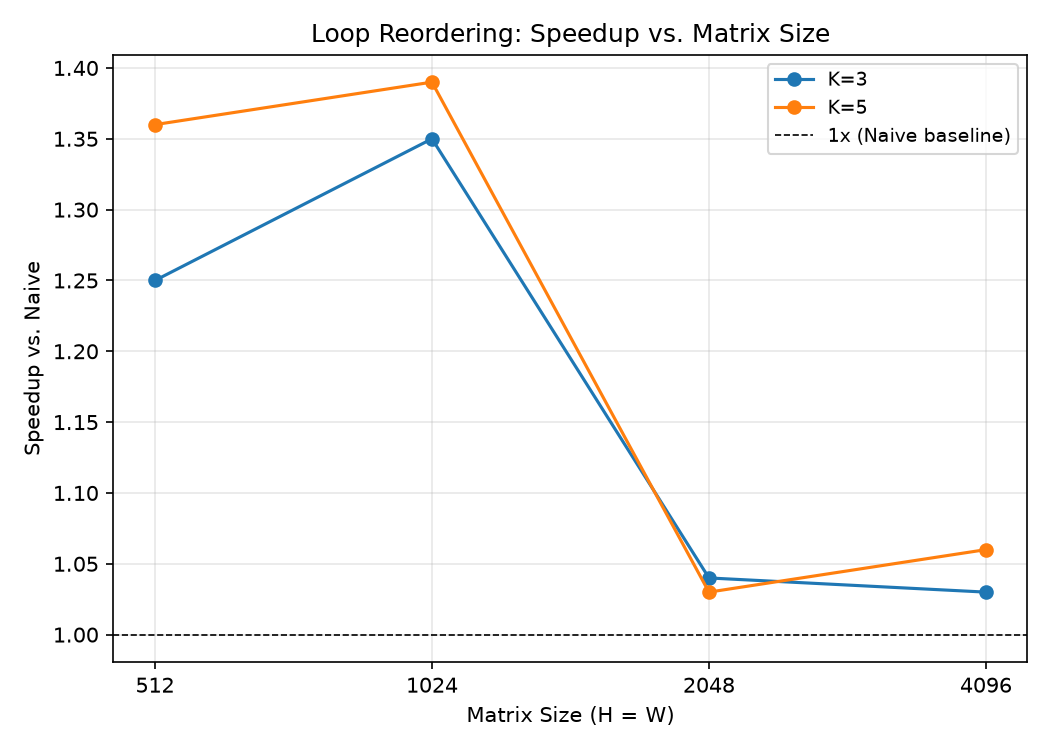
\includegraphics[width=0.7\textwidth]{figures/speedup_vs_size_reorder.png}
  \caption{Loop Reordering: speedup vs.\ matrix size, $K=3$ and $K=5$.}
\end{figure}

\subsubsection*{Loop Unrolling --- Best (16 Accumulators)}
\begin{table}[H]
  \centering
  \caption{16-wide Unroll (16 Accumulators)}
  \label{tab:unroll_unrolling8combo_16acc}
  \resizebox{\textwidth}{!}{%
  \begin{tabular}{lcccccccccc}
    \toprule
    Image Size ($H \times W$) & \multicolumn{5}{c}{$K=3$} & \multicolumn{5}{c}{$K=5$} \\
    \cmidrule(lr){2-6} \cmidrule(lr){7-11}
     & Time (ms) & GFLOP/s & Speedup & Isolated Instr. (M) & Isolated MPKI & Time (ms) & GFLOP/s & Speedup & Isolated Instr. (M) & Isolated MPKI \\
    \midrule
    $512 \times 512$ & 0.311 & 15.16 & 3.18$\times$ & 45.44 & 8.007 & 0.850 & 15.43 & 3.63$\times$ & 103.29 & 3.531 \\
    $1024 \times 1024$ & 1.303 & 14.49 & 3.59$\times$ & 181.07 & 8.007 & 3.404 & 15.40 & 4.01$\times$ & 413.45 & 3.564 \\
    $2048 \times 2048$ & 5.534 & 13.64 & 3.75$\times$ & 724.19 & 8.101 & 14.263 & 14.70 & 3.92$\times$ & 1652.38 & 5.320 \\
    $4096 \times 4096$ & 22.584 & 13.37 & 3.63$\times$ & 3061.73 & 13.762 & 57.133 & 14.68 & 3.91$\times$ & 6638.23 & 9.797 \\
    \bottomrule
  \end{tabular}
  }
\end{table}

\begin{figure}[H]
  \centering
  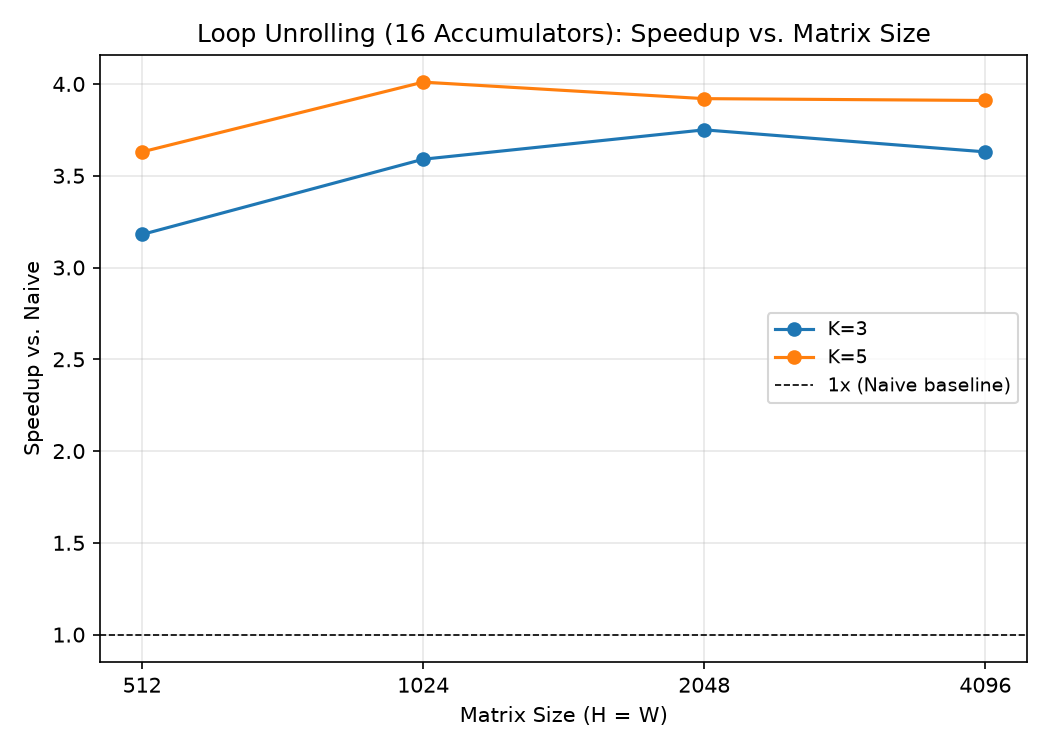
\includegraphics[width=0.7\textwidth]{figures/speedup_vs_size_unroll.png}
  \caption{Loop Unrolling (16 accumulators): speedup vs.\ matrix size, $K=3$ and $K=5$.}
\end{figure}

\subsection*{Alternate Runs (Loop Unrolling)}

\begin{table}[H]
  \centering
  \caption{8-wide Unroll}
  \label{tab:unroll_unrolling8combo}
  \resizebox{\textwidth}{!}{%
  \begin{tabular}{lcccccccccc}
    \toprule
    Image Size ($H \times W$) & \multicolumn{5}{c}{$K=3$} & \multicolumn{5}{c}{$K=5$} \\
    \cmidrule(lr){2-6} \cmidrule(lr){7-11}
     & Time (ms) & GFLOP/s & Speedup & Isolated Instr. (M) & Isolated MPKI & Time (ms) & GFLOP/s & Speedup & Isolated Instr. (M) & Isolated MPKI \\
    \midrule
    $512 \times 512$ & 0.334 & 14.14 & 3.02$\times$ & 59.67 & 6.017 & 0.897 & 14.62 & 3.40$\times$ & 133.56 & 2.705 \\
    $1024 \times 1024$ & 1.397 & 13.51 & 3.21$\times$ & 238.27 & 6.051 & 3.743 & 14.01 & 3.54$\times$ & 534.31 & 2.761 \\
    $2048 \times 2048$ & 6.618 & 11.41 & 3.12$\times$ & 952.13 & 6.235 & 17.498 & 11.99 & 3.12$\times$ & 2137.28 & 5.047 \\
    $4096 \times 4096$ & 24.420 & 12.37 & 3.26$\times$ & 3992.44 & 10.563 & 61.804 & 13.57 & 3.54$\times$ & 8662.83 & 7.441 \\
    \bottomrule
  \end{tabular}
  }
\end{table}

\subsection{Discussion}
Loop reordering alone achieves only a modest and inconsistent speedup (roughly
$1.0$--$1.4\times$ across sizes), while loop unrolling with 16 accumulators achieves a
much larger and more consistent speedup (roughly $3.2$--$3.7\times$). This is consistent
with the two techniques targeting different bottlenecks: reordering changes memory
\emph{access pattern} without reducing the number of instructions executed or the length
of the accumulator's dependency chain, whereas unrolling directly shortens that
dependency chain (multiple independent accumulators can be summed by the CPU in
parallel rather than serially) and amortizes loop-overhead instructions (index increment,
bound check, branch) across more useful work per iteration. The 16-accumulator variant
outperforms the plain 8-wide combined-accumulator variant, supporting the expectation that
more independent accumulators better hide floating-point addition/FMA latency.

\section{Task 1B: Tiling}
\subsection{L1-D Cache Size}
As mentioned above, the L1-D Cache of the machine this task was tested on is 48 KiB.

\subsection{Tiled Implementation}
The tiled implementation blocks the output computation into \texttt{tile\_size} $\times$ \texttt{tile\_size} regions, iterating \texttt{Ty}/\texttt{Tx} over tiles and \texttt{oy}/\texttt{ox} within each tile, so that the input rows touched by one tile are more likely to still be cache-resident across the $K \times K$ kernel taps for nearby output pixels. \texttt{tile\_size} is a compile-time constant in \texttt{conv\_tile.cpp}; each tile size below required a manual edit and rebuild between runs (values tested: 8, 16, 32, 64, 128, 256, 512, 1024).

\subsection{Best Tile Size: Tile=256}
\begin{table}[H]
  \centering
  \caption{Tile Size = 256}
  \label{tab:tile_tileSize256}
  \resizebox{\textwidth}{!}{%
  \begin{tabular}{lcccccccccc}
    \toprule
    Image Size ($H \times W$) & \multicolumn{5}{c}{$K=3$} & \multicolumn{5}{c}{$K=5$} \\
    \cmidrule(lr){2-6} \cmidrule(lr){7-11}
     & Time (ms) & GFLOP/s & Speedup & Isolated Instr. (M) & Isolated MPKI & Time (ms) & GFLOP/s & Speedup & Isolated Instr. (M) & Isolated MPKI \\
    \midrule
    $512 \times 512$ & 1.002 & 4.71 & 1.03$\times$ & 233.04 & 1.703 & 3.401 & 3.85 & 0.94$\times$ & 526.85 & 0.780 \\
    $1024 \times 1024$ & 4.449 & 4.24 & 1.05$\times$ & 932.60 & 1.741 & 14.931 & 3.51 & 0.92$\times$ & 2107.76 & 0.791 \\
    $2048 \times 2048$ & 19.391 & 3.89 & 1.06$\times$ & 3731.17 & 1.753 & 58.957 & 3.56 & 0.96$\times$ & 8431.48 & 0.776 \\
    $4096 \times 4096$ & 77.437 & 3.90 & 1.05$\times$ & 14924.45 & 1.709 & 227.466 & 3.69 & 0.98$\times$ & 33725.20 & 0.769 \\
    \bottomrule
  \end{tabular}
  }
\end{table}
\subsection*{Alternate Runs (Other Tile Sizes)}

\begin{table}[H]
  \centering
  \caption{Tile Size = 8}
  \label{tab:tile_tileSize8}
  \resizebox{\textwidth}{!}{%
  \begin{tabular}{lcccccccccc}
    \toprule
    Image Size ($H \times W$) & \multicolumn{5}{c}{$K=3$} & \multicolumn{5}{c}{$K=5$} \\
    \cmidrule(lr){2-6} \cmidrule(lr){7-11}
     & Time (ms) & GFLOP/s & Speedup & Isolated Instr. (M) & Isolated MPKI & Time (ms) & GFLOP/s & Speedup & Isolated Instr. (M) & Isolated MPKI \\
    \midrule
    $512 \times 512$ & 1.072 & 4.40 & 0.93$\times$ & 243.60 & 1.554 & 3.401 & 3.85 & 0.94$\times$ & 537.30 & 0.798 \\
    $1024 \times 1024$ & 5.119 & 3.69 & 0.91$\times$ & 974.58 & 1.940 & 15.729 & 3.33 & 0.97$\times$ & 2149.68 & 1.114 \\
    $2048 \times 2048$ & 21.035 & 3.59 & 1.00$\times$ & 3897.62 & 1.960 & 58.775 & 3.57 & 0.96$\times$ & 8597.62 & 1.085 \\
    $4096 \times 4096$ & 82.181 & 3.67 & 1.01$\times$ & 15590.02 & 1.876 & 232.968 & 3.60 & 0.97$\times$ & 34390.86 & 1.038 \\
    \bottomrule
  \end{tabular}
  }
\end{table}

\begin{table}[H]
  \centering
  \caption{Tile Size = 16}
  \label{tab:tile_tileSize16}
  \resizebox{\textwidth}{!}{%
  \begin{tabular}{lcccccccccc}
    \toprule
    Image Size ($H \times W$) & \multicolumn{5}{c}{$K=3$} & \multicolumn{5}{c}{$K=5$} \\
    \cmidrule(lr){2-6} \cmidrule(lr){7-11}
     & Time (ms) & GFLOP/s & Speedup & Isolated Instr. (M) & Isolated MPKI & Time (ms) & GFLOP/s & Speedup & Isolated Instr. (M) & Isolated MPKI \\
    \midrule
    $512 \times 512$ & 1.087 & 4.34 & 0.92$\times$ & 246.16 & 1.730 & 3.919 & 3.34 & 0.91$\times$ & 545.16 & 0.847 \\
    $1024 \times 1024$ & 5.051 & 3.74 & 1.16$\times$ & 984.81 & 3.770 & 15.673 & 3.35 & 0.90$\times$ & 2180.99 & 1.264 \\
    $2048 \times 2048$ & 22.730 & 3.32 & 0.98$\times$ & 3939.00 & 3.768 & 61.436 & 3.41 & 1.02$\times$ & 8723.60 & 1.251 \\
    $4096 \times 4096$ & 81.916 & 3.69 & 1.01$\times$ & 15755.40 & 3.737 & 238.551 & 3.52 & 0.94$\times$ & 34891.30 & 1.243 \\
    \bottomrule
  \end{tabular}
  }
\end{table}

\begin{table}[H]
  \centering
  \caption{Tile Size = 32}
  \label{tab:tile_tileSize32}
  \resizebox{\textwidth}{!}{%
  \begin{tabular}{lcccccccccc}
    \toprule
    Image Size ($H \times W$) & \multicolumn{5}{c}{$K=3$} & \multicolumn{5}{c}{$K=5$} \\
    \cmidrule(lr){2-6} \cmidrule(lr){7-11}
     & Time (ms) & GFLOP/s & Speedup & Isolated Instr. (M) & Isolated MPKI & Time (ms) & GFLOP/s & Speedup & Isolated Instr. (M) & Isolated MPKI \\
    \midrule
    $512 \times 512$ & 1.090 & 4.33 & 0.90$\times$ & 243.29 & 2.514 & 3.421 & 3.83 & 0.94$\times$ & 542.35 & 0.896 \\
    $1024 \times 1024$ & 4.947 & 3.82 & 0.94$\times$ & 973.58 & 2.686 & 15.961 & 3.28 & 0.86$\times$ & 2169.73 & 1.148 \\
    $2048 \times 2048$ & 20.558 & 3.67 & 0.98$\times$ & 3894.35 & 2.656 & 58.109 & 3.61 & 1.06$\times$ & 8678.30 & 1.133 \\
    $4096 \times 4096$ & 81.741 & 3.69 & 0.96$\times$ & 15577.31 & 2.625 & 230.608 & 3.64 & 0.96$\times$ & 34713.61 & 1.126 \\
    \bottomrule
  \end{tabular}
  }
\end{table}

\begin{table}[H]
  \centering
  \caption{Tile Size = 64}
  \label{tab:tile_tileSize64}
  \resizebox{\textwidth}{!}{%
  \begin{tabular}{lcccccccccc}
    \toprule
    Image Size ($H \times W$) & \multicolumn{5}{c}{$K=3$} & \multicolumn{5}{c}{$K=5$} \\
    \cmidrule(lr){2-6} \cmidrule(lr){7-11}
     & Time (ms) & GFLOP/s & Speedup & Isolated Instr. (M) & Isolated MPKI & Time (ms) & GFLOP/s & Speedup & Isolated Instr. (M) & Isolated MPKI \\
    \midrule
    $512 \times 512$ & 1.065 & 4.43 & 0.93$\times$ & 241.99 & 2.055 & 3.392 & 3.86 & 0.95$\times$ & 540.88 & 0.905 \\
    $1024 \times 1024$ & 4.823 & 3.91 & 1.00$\times$ & 968.35 & 2.100 & 15.076 & 3.48 & 1.00$\times$ & 2164.47 & 0.948 \\
    $2048 \times 2048$ & 20.479 & 3.69 & 0.99$\times$ & 3872.75 & 2.099 & 60.879 & 3.44 & 0.92$\times$ & 8657.06 & 0.931 \\
    $4096 \times 4096$ & 81.854 & 3.69 & 0.99$\times$ & 15490.85 & 2.064 & 229.256 & 3.66 & 0.97$\times$ & 34626.79 & 0.930 \\
    \bottomrule
  \end{tabular}
  }
\end{table}

\begin{table}[H]
  \centering
  \caption{Tile Size = 128}
  \label{tab:tile_tileSize128}
  \resizebox{\textwidth}{!}{%
  \begin{tabular}{lcccccccccc}
    \toprule
    Image Size ($H \times W$) & \multicolumn{5}{c}{$K=3$} & \multicolumn{5}{c}{$K=5$} \\
    \cmidrule(lr){2-6} \cmidrule(lr){7-11}
     & Time (ms) & GFLOP/s & Speedup & Isolated Instr. (M) & Isolated MPKI & Time (ms) & GFLOP/s & Speedup & Isolated Instr. (M) & Isolated MPKI \\
    \midrule
    $512 \times 512$ & 1.052 & 4.49 & 0.94$\times$ & 241.27 & 1.784 & 3.351 & 3.91 & 0.94$\times$ & 540.29 & 0.843 \\
    $1024 \times 1024$ & 4.727 & 3.99 & 0.99$\times$ & 965.74 & 1.867 & 14.783 & 3.55 & 0.95$\times$ & 2161.74 & 0.826 \\
    $2048 \times 2048$ & 21.386 & 3.53 & 0.98$\times$ & 3862.18 & 1.831 & 58.765 & 3.57 & 0.97$\times$ & 8646.68 & 0.830 \\
    $4096 \times 4096$ & 81.697 & 3.70 & 0.99$\times$ & 15448.56 & 1.795 & 227.959 & 3.68 & 0.98$\times$ & 34584.23 & 0.805 \\
    \bottomrule
  \end{tabular}
  }
\end{table}

\begin{table}[H]
  \centering
  \caption{Tile Size = 512}
  \label{tab:tile_tileSize512}
  \resizebox{\textwidth}{!}{%
  \begin{tabular}{lcccccccccc}
    \toprule
    Image Size ($H \times W$) & \multicolumn{5}{c}{$K=3$} & \multicolumn{5}{c}{$K=5$} \\
    \cmidrule(lr){2-6} \cmidrule(lr){7-11}
     & Time (ms) & GFLOP/s & Speedup & Isolated Instr. (M) & Isolated MPKI & Time (ms) & GFLOP/s & Speedup & Isolated Instr. (M) & Isolated MPKI \\
    \midrule
    $512 \times 512$ & 1.031 & 4.58 & 0.95$\times$ & 232.99 & 1.571 & 3.406 & 3.85 & 0.93$\times$ & 528.61 & 0.820 \\
    $1024 \times 1024$ & 4.680 & 4.03 & 0.97$\times$ & 932.11 & 1.643 & 15.215 & 3.45 & 0.93$\times$ & 2107.49 & 0.776 \\
    $2048 \times 2048$ & 19.809 & 3.81 & 1.03$\times$ & 3728.36 & 1.677 & 60.193 & 3.48 & 0.96$\times$ & 8428.96 & 0.803 \\
    $4096 \times 4096$ & 77.230 & 3.91 & 1.06$\times$ & 14913.28 & 1.639 & 227.665 & 3.68 & 0.99$\times$ & 33713.92 & 0.745 \\
    \bottomrule
  \end{tabular}
  }
\end{table}

\begin{table}[H]
  \centering
  \caption{Tile Size = 1024}
  \label{tab:tile_tileSize1024}
  \resizebox{\textwidth}{!}{%
  \begin{tabular}{lcccccccccc}
    \toprule
    Image Size ($H \times W$) & \multicolumn{5}{c}{$K=3$} & \multicolumn{5}{c}{$K=5$} \\
    \cmidrule(lr){2-6} \cmidrule(lr){7-11}
     & Time (ms) & GFLOP/s & Speedup & Isolated Instr. (M) & Isolated MPKI & Time (ms) & GFLOP/s & Speedup & Isolated Instr. (M) & Isolated MPKI \\
    \midrule
    $512 \times 512$ & 0.981 & 4.81 & 1.01$\times$ & 233.04 & 1.552 & 3.383 & 3.87 & 0.92$\times$ & 526.63 & 0.711 \\
    $1024 \times 1024$ & 4.452 & 4.24 & 1.02$\times$ & 932.06 & 1.604 & 14.815 & 3.54 & 0.95$\times$ & 2107.08 & 0.761 \\
    $2048 \times 2048$ & 20.287 & 3.72 & 1.02$\times$ & 3727.04 & 1.651 & 57.771 & 3.63 & 1.02$\times$ & 8427.72 & 0.822 \\
    $4096 \times 4096$ & 77.867 & 3.88 & 1.05$\times$ & 14908.31 & 1.611 & 226.613 & 3.70 & 0.98$\times$ & 33707.90 & 0.747 \\
    \bottomrule
  \end{tabular}
  }
\end{table}

\subsection{Figures}
\begin{figure}[H]
  \centering
  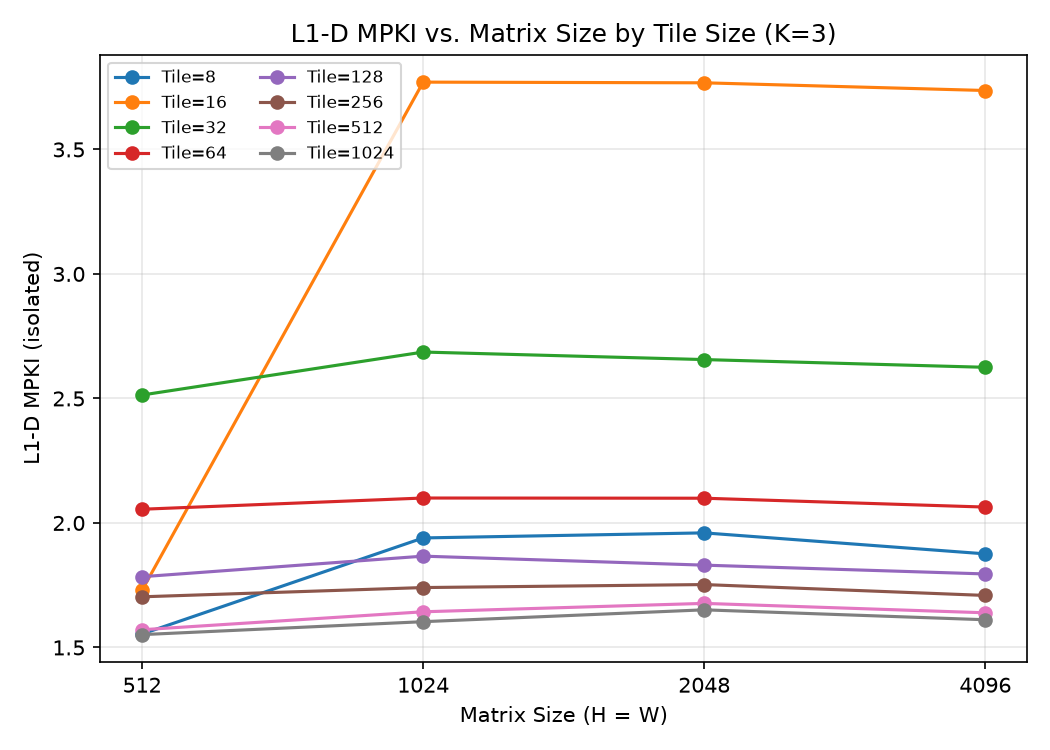
\includegraphics[width=0.8\textwidth]{figures/mpki_vs_size_tile_K3.png}
  \caption{L1-D MPKI vs.\ matrix size, by tile size ($K=3$).}
\end{figure}
\begin{figure}[H]
  \centering
  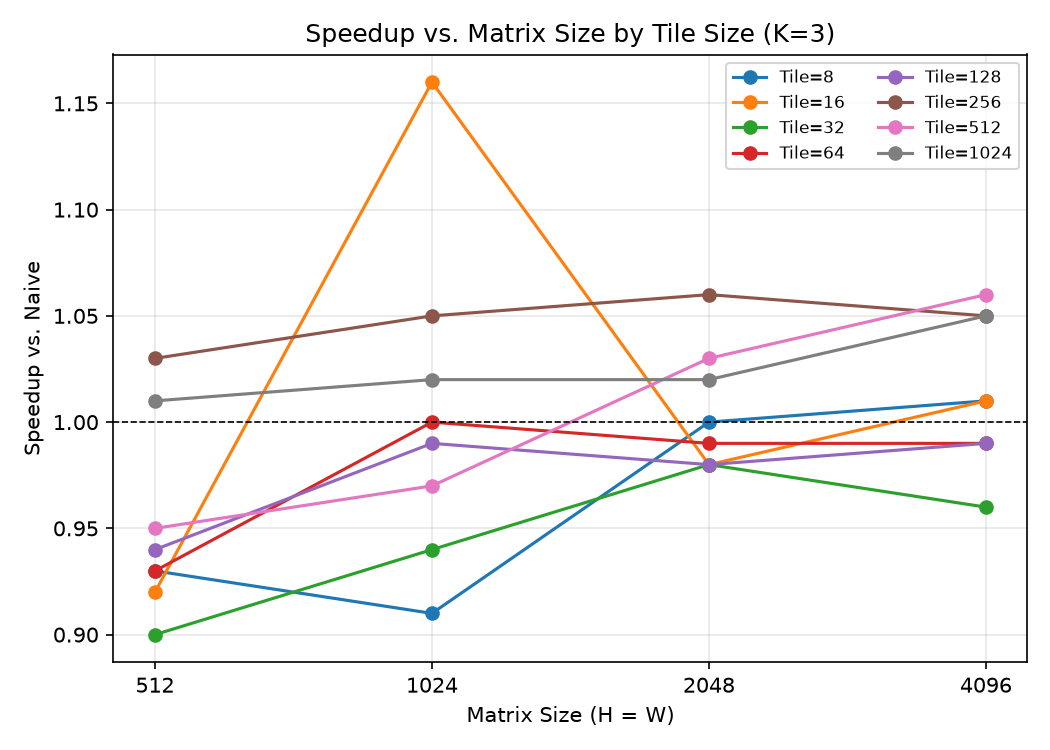
\includegraphics[width=0.8\textwidth]{figures/speedup_vs_size_tile_K3.png}
  \caption{Speedup vs.\ matrix size, by tile size ($K=3$).}
\end{figure}


\subsection{Answers}

\paragraph{Q1: Change in L1-D MPKI, naive $\to$ tiled.}
The reduction in MKPI seems to be reducing as the size of the Image Increases as expected from Tiling, as for larger images which will not fit in the cache, the additional code causes relatively low overhead in favour of increased hits in the L1-D Cache.

\paragraph{Q2: MPKI vs.\ matrix size and tile size.}
Across all the runs that were conducted, the MPKI is roughly similar across all the tile sizes as expected since the tiling keeps it's working set same regarded image size. Rather another way to explain this can be that the L1 Misses and and the Number of Instructions are growing at the same rate, with the only one outlier being at Tile Size 16

\paragraph{Q3: Did tiling alone achieve a speedup?}


In all of the Runs performed, we observed that Tiling only rarely gave a overall speedup, with many a times being a performance degrade. We also noticed that the speedup is highly inconsistent with one example shown below:

$ taskset -c 7 ./bin/conv tile 256 256 3 1234

CS683 PA-1 Task 1  2D convolution optimization harness

=== Workload  H=256 W=256 K=3 seed=1234 (not graded) ===
stage           correct    time(ms)     GFLOP/s    speedup
--------------------------------------------------------------
naive (ref)     yes           0.279        4.23      1.00x
tile            yes           0.274        4.30      1.02x


$ taskset -c 7 ./bin/conv tile 256 256 3 1234

CS683 PA-1 Task 1  2D convolution optimization harness

=== Workload  H=256 W=256 K=3 seed=1234 (not graded) ===
stage           correct    time(ms)     GFLOP/s    speedup
--------------------------------------------------------------
naive (ref)     yes           0.592        1.99      1.00x
tile            yes           0.277        4.26      2.14x

These 2 runs were performed in somewhat of a quick sucession. We are unsure of the 2.14x in the second attempt. Furthermore, while in the 2-3 minutes of discussing this dilemma:

$ taskset -c 7 ./bin/conv tile 256 256 3 1234

CS683 PA-1 Task 1  2D convolution optimization harness

=== Workload  H=256 W=256 K=3 seed=1234 (not graded) ===
stage           correct    time(ms)     GFLOP/s    speedup
--------------------------------------------------------------
naive (ref)     yes           0.612        1.93      1.00x
tile            yes           0.272        4.34      2.25x

Here the speedup is still 2.25x but then not in the subsequent run. Further more, late into the assignment we also observed that Turning the Hardware Prefetcher off seemed to perform consistently better. We are unsure of the reasons of these discrepancies and decided to document this.



\section{Task 1C: SIMD}

\subsection{Baseline Instruction Count}
The naive implementation's instruction count (from the dedicated baseline \texttt{perf} run, Table~\ref{tab:naive_n8combo}) grows from $\sim$278.5M instructions at $512\times512$, $K{=}3$ up to $\sim$17.2 billion at $4096\times4096$, $K{=}3$ (and correspondingly higher for $K{=}5$, e.g.\ $\sim$601.6M at $512\times512$ up to $\sim$37.9 billion at $4096\times4096$).

\subsection{SIMD Implementation}
Versions were implemented at 128-bit (4 floats/register), 256-bit (8 floats/register), and 512-bit (16
floats/register) widths, each with the kernel weight broadcast via \verb|set1_ps| and loads and stores were done via \verb|load_ps| and \verb|load_ps| due to the Inputs and Outputs being aligned. Several unroll-width variants per SIMD width (1x/2x/4x processing multiple vector chunks per output-row iteration) were also tested to explore instruction-level parallelism.

\subsection{Best SIMD Configuration: 256-bit, 2x Unroll}
\begin{table}[H]
  \centering
  \caption{256-bit SIMD, 2x Unroll}
  \label{tab:simd_256bits2unroll}
  \resizebox{\textwidth}{!}{%
  \begin{tabular}{lcccccccccc}
    \toprule
    Image Size ($H \times W$) & \multicolumn{5}{c}{$K=3$} & \multicolumn{5}{c}{$K=5$} \\
    \cmidrule(lr){2-6} \cmidrule(lr){7-11}
     & Time (ms) & GFLOP/s & Speedup & Isolated Instr. (M) & Isolated MPKI & Time (ms) & GFLOP/s & Speedup & Isolated Instr. (M) & Isolated MPKI \\
    \midrule
    $512 \times 512$ & 0.080 & 58.99 & 12.51$\times$ & 19.50 & 18.517 & 0.211 & 62.07 & 14.58$\times$ & 40.86 & 8.898 \\
    $1024 \times 1024$ & 0.333 & 56.63 & 14.43$\times$ & 78.11 & 18.532 & 0.888 & 59.02 & 15.46$\times$ & 163.17 & 9.099 \\
    $2048 \times 2048$ & 2.007 & 37.62 & 10.57$\times$ & 311.97 & 19.208 & 4.500 & 46.60 & 12.81$\times$ & 653.17 & 13.584 \\
    $4096 \times 4096$ & 9.841 & 30.69 & 8.58$\times$ & 1257.76 & 32.632 & 18.155 & 46.21 & 12.45$\times$ & 2612.12 & 25.008 \\
    \bottomrule
  \end{tabular}
  }
\end{table}
\subsection*{Alternate Runs (Other SIMD Widths/Unroll Factors)}

\begin{table}[H]
  \centering
  \caption{128-bit SIMD, 1x Unroll}
  \label{tab:simd_128bits1unroll}
  \resizebox{\textwidth}{!}{%
  \begin{tabular}{lcccccccccc}
    \toprule
    Image Size ($H \times W$) & \multicolumn{5}{c}{$K=3$} & \multicolumn{5}{c}{$K=5$} \\
    \cmidrule(lr){2-6} \cmidrule(lr){7-11}
     & Time (ms) & GFLOP/s & Speedup & Isolated Instr. (M) & Isolated MPKI & Time (ms) & GFLOP/s & Speedup & Isolated Instr. (M) & Isolated MPKI \\
    \midrule
    $512 \times 512$ & 0.241 & 19.56 & 4.11$\times$ & 53.88 & 6.702 & 0.840 & 15.60 & 3.80$\times$ & 116.91 & 3.164 \\
    $1024 \times 1024$ & 1.062 & 17.77 & 4.49$\times$ & 215.92 & 6.734 & 3.418 & 15.34 & 4.00$\times$ & 467.43 & 3.211 \\
    $2048 \times 2048$ & 4.900 & 15.41 & 4.45$\times$ & 862.92 & 6.877 & 14.493 & 14.47 & 3.94$\times$ & 1869.97 & 5.276 \\
    $4096 \times 4096$ & 19.055 & 15.85 & 4.39$\times$ & 3469.39 & 10.818 & 56.315 & 14.90 & 3.98$\times$ & 7479.28 & 8.741 \\
    \bottomrule
  \end{tabular}
  }
\end{table}

\begin{table}[H]
  \centering
  \caption{128-bit SIMD, 2x Unroll}
  \label{tab:simd_128bits2unroll}
  \resizebox{\textwidth}{!}{%
  \begin{tabular}{lcccccccccc}
    \toprule
    Image Size ($H \times W$) & \multicolumn{5}{c}{$K=3$} & \multicolumn{5}{c}{$K=5$} \\
    \cmidrule(lr){2-6} \cmidrule(lr){7-11}
     & Time (ms) & GFLOP/s & Speedup & Isolated Instr. (M) & Isolated MPKI & Time (ms) & GFLOP/s & Speedup & Isolated Instr. (M) & Isolated MPKI \\
    \midrule
    $512 \times 512$ & 0.149 & 31.75 & 8.04$\times$ & 39.50 & 9.154 & 0.425 & 30.87 & 7.28$\times$ & 84.05 & 4.346 \\
    $1024 \times 1024$ & 0.644 & 29.31 & 7.07$\times$ & 158.08 & 9.181 & 1.789 & 29.31 & 7.65$\times$ & 336.53 & 4.460 \\
    $2048 \times 2048$ & 3.061 & 24.66 & 7.02$\times$ & 632.19 & 9.452 & 7.753 & 27.05 & 7.48$\times$ & 1345.75 & 7.618 \\
    $4096 \times 4096$ & 13.044 & 23.15 & 6.20$\times$ & 2526.96 & 15.235 & 33.910 & 24.74 & 6.58$\times$ & 5382.12 & 12.117 \\
    \bottomrule
  \end{tabular}
  }
\end{table}

\begin{table}[H]
  \centering
  \caption{128-bit SIMD, 4x Unroll}
  \label{tab:simd_128bits4unroll}
  \resizebox{\textwidth}{!}{%
  \begin{tabular}{lcccccccccc}
    \toprule
    Image Size ($H \times W$) & \multicolumn{5}{c}{$K=3$} & \multicolumn{5}{c}{$K=5$} \\
    \cmidrule(lr){2-6} \cmidrule(lr){7-11}
     & Time (ms) & GFLOP/s & Speedup & Isolated Instr. (M) & Isolated MPKI & Time (ms) & GFLOP/s & Speedup & Isolated Instr. (M) & Isolated MPKI \\
    \midrule
    $512 \times 512$ & 0.103 & 45.62 & 9.97$\times$ & 25.18 & 14.420 & 0.323 & 40.58 & 9.44$\times$ & 53.05 & 6.857 \\
    $1024 \times 1024$ & 0.438 & 43.05 & 10.49$\times$ & 100.63 & 14.435 & 1.202 & 43.64 & 11.38$\times$ & 212.04 & 7.201 \\
    $2048 \times 2048$ & 2.190 & 34.48 & 10.62$\times$ & 401.28 & 15.334 & 5.784 & 36.26 & 9.79$\times$ & 847.13 & 10.683 \\
    $4096 \times 4096$ & 11.010 & 27.43 & 8.07$\times$ & 1604.60 & 25.323 & 23.504 & 35.69 & 9.40$\times$ & 3388.51 & 19.238 \\
    \bottomrule
  \end{tabular}
  }
\end{table}

\begin{table}[H]
  \centering
  \caption{256-bit SIMD, 1x Unroll}
  \label{tab:simd_256bits1unroll}
  \resizebox{\textwidth}{!}{%
  \begin{tabular}{lcccccccccc}
    \toprule
    Image Size ($H \times W$) & \multicolumn{5}{c}{$K=3$} & \multicolumn{5}{c}{$K=5$} \\
    \cmidrule(lr){2-6} \cmidrule(lr){7-11}
     & Time (ms) & GFLOP/s & Speedup & Isolated Instr. (M) & Isolated MPKI & Time (ms) & GFLOP/s & Speedup & Isolated Instr. (M) & Isolated MPKI \\
    \midrule
    $512 \times 512$ & 0.125 & 37.68 & 7.85$\times$ & 28.01 & 12.861 & 0.448 & 29.28 & 7.05$\times$ & 59.51 & 6.513 \\
    $1024 \times 1024$ & 0.545 & 34.63 & 8.92$\times$ & 112.32 & 12.917 & 1.782 & 29.43 & 7.78$\times$ & 237.98 & 6.418 \\
    $2048 \times 2048$ & 2.877 & 26.24 & 7.67$\times$ & 448.64 & 13.330 & 7.794 & 26.91 & 7.40$\times$ & 952.41 & 10.531 \\
    $4096 \times 4096$ & 11.826 & 25.54 & 7.10$\times$ & 1793.18 & 22.729 & 31.536 & 26.60 & 7.22$\times$ & 3808.89 & 17.157 \\
    \bottomrule
  \end{tabular}
  }
\end{table}

\begin{table}[H]
  \centering
  \caption{512-bit SIMD, 1x Unroll}
  \label{tab:simd_512bits1unroll}
  \resizebox{\textwidth}{!}{%
  \begin{tabular}{lcccccccccc}
    \toprule
    Image Size ($H \times W$) & \multicolumn{5}{c}{$K=3$} & \multicolumn{5}{c}{$K=5$} \\
    \cmidrule(lr){2-6} \cmidrule(lr){7-11}
     & Time (ms) & GFLOP/s & Speedup & Isolated Instr. (M) & Isolated MPKI & Time (ms) & GFLOP/s & Speedup & Isolated Instr. (M) & Isolated MPKI \\
    \midrule
    $512 \times 512$ & 0.097 & 48.63 & 10.82$\times$ & 14.97 & 23.830 & 0.238 & 55.05 & 14.43$\times$ & 30.83 & 11.928 \\
    $1024 \times 1024$ & 0.343 & 55.00 & 14.77$\times$ & 60.51 & 23.899 & 0.910 & 57.60 & 15.30$\times$ & 123.37 & 12.002 \\
    $2048 \times 2048$ & 1.958 & 38.55 & 10.63$\times$ & 240.84 & 24.142 & 4.568 & 45.91 & 12.95$\times$ & 492.67 & 17.111 \\
    $4096 \times 4096$ & 9.671 & 31.23 & 9.39$\times$ & 964.54 & 43.459 & 17.397 & 48.22 & 12.73$\times$ & 1972.28 & 33.042 \\
    \bottomrule
  \end{tabular}
  }
\end{table}

\subsection{Figure}
\begin{figure}[H]
  \centering
  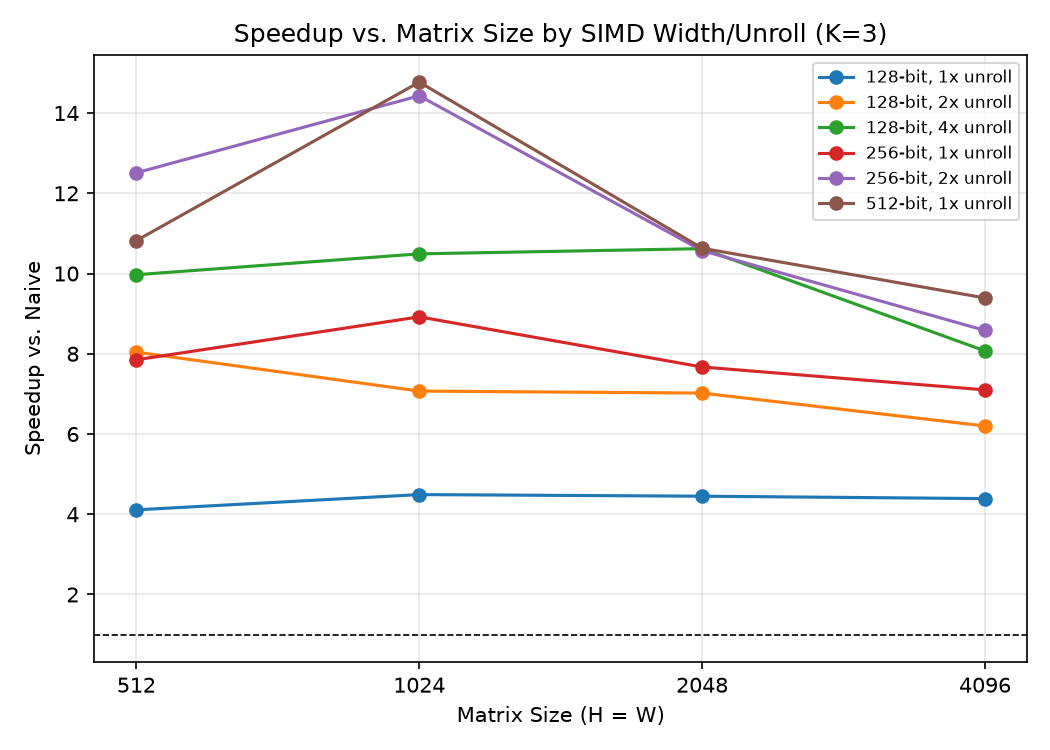
\includegraphics[width=0.8\textwidth]{figures/speedup_vs_size_simd_K3.png}
  \caption{Speedup vs.\ matrix size, by SIMD width/unroll factor ($K=3$).}
\end{figure}


\subsection{Answers}

\paragraph{Q1: Change in instruction count, naive $\to$ SIMD.}
As reported on the Tables above, using SIMD reduced the Instruction Count significantly. This is pretty straight forward observation as the number of individual operations being packed into 1 individual would dramatically reduce the total number of Instructions.

\paragraph{Q2: Speedup achieved.}
The performance increase (atleast for 1x Unroll), seems to be dependent on the type of Width used, with 128-bit having roughly 4x, 256-bit having roughly 7.5x-8x and roughly 11x-12x for 512-bit.

\paragraph{Q3: SIMD intrinsics used and justification.}
\texttt{\_mm\{,256,512\}\_set1\_ps} to broadcast each scalar kernel weight across the vector register, \texttt{\_mm\{,256,512\}\_load\_ps} / \texttt{\_mm\{,256,512\}\_store\_ps} for input/output access, chosen due to the Input and output being aligned although it is safer to use the unaligned version if this wasn't known, and texttt{\_mm\{,256,512\}\_fmadd\_ps} to fuse the multiply and accumulate into a single instruction, reducing the instruction count.

\section{Task 1D: Final Optimized (Unrolling + Tiling + SIMD) (Teeno Ka Saath, Marks ka Vikaas)}

\subsection{Implementation}
The final optimized kernel combines Unrolling (Task 1A), cache tiling (Task 1B) with SIMD vectorization
(Task 1C). Both \texttt{tile\_size} and the SIMD width were swept manually
(tile sizes 16/32/64 $\times$ SIMD widths 128/256/512-bit, 9 configurations total).
Per the sweep results, \texttt{Tile=32} paired with either 256-bit or 512-bit SIMD gives
the most \emph{consistently} strong result: both stay above $8\times$ speedup at every
matrix size tested, which is not true of every configuration (e.g.\ \texttt{Tile=64} with
512-bit SIMD has the single highest average speedup, but dips to $8.41\times$ at its worst
case -- Tile=32 is the more robust choice). Both Tile=32 configurations are presented as
co-primary results below.

\subsection{Results}

\subsubsection*{Tile=32, 512-bit SIMD (highest average speedup)}
\begin{table}[H]
  \centering
  \caption{Tile Size = 32, 512-bit SIMD}
  \label{tab:optimized_tileSize32SIMDbits512}
  \resizebox{\textwidth}{!}{%
  \begin{tabular}{lcccccccccc}
    \toprule
    Image Size ($H \times W$) & \multicolumn{5}{c}{$K=3$} & \multicolumn{5}{c}{$K=5$} \\
    \cmidrule(lr){2-6} \cmidrule(lr){7-11}
     & Time (ms) & GFLOP/s & Speedup & Isolated Instr. (M) & Isolated MPKI & Time (ms) & GFLOP/s & Speedup & Isolated Instr. (M) & Isolated MPKI \\
    \midrule
    $512 \times 512$ & 0.079 & 59.40 & 12.58$\times$ & 12.14 & 41.928 & 0.202 & 64.75 & 15.04$\times$ & 23.32 & 19.609 \\
    $1024 \times 1024$ & 0.345 & 54.70 & 13.45$\times$ & 48.92 & 43.856 & 0.741 & 70.76 & 18.35$\times$ & 93.70 & 24.576 \\
    $2048 \times 2048$ & 2.113 & 35.73 & 10.43$\times$ & 196.31 & 43.938 & 3.417 & 61.38 & 16.58$\times$ & 374.10 & 24.619 \\
    $4096 \times 4096$ & 9.169 & 32.94 & 9.54$\times$ & 816.67 & 41.193 & 14.277 & 58.76 & 15.64$\times$ & 1498.04 & 24.466 \\
    \bottomrule
  \end{tabular}
  }
\end{table}
\subsubsection*{Tile=32, 256-bit SIMD (co-primary --- also consistently $>8\times$)}
\begin{table}[H]
  \centering
  \caption{Tile Size = 32, 256-bit SIMD}
  \label{tab:optimized_tileSize32SIMDbits256}
  \resizebox{\textwidth}{!}{%
  \begin{tabular}{lcccccccccc}
    \toprule
    Image Size ($H \times W$) & \multicolumn{5}{c}{$K=3$} & \multicolumn{5}{c}{$K=5$} \\
    \cmidrule(lr){2-6} \cmidrule(lr){7-11}
     & Time (ms) & GFLOP/s & Speedup & Isolated Instr. (M) & Isolated MPKI & Time (ms) & GFLOP/s & Speedup & Isolated Instr. (M) & Isolated MPKI \\
    \midrule
    $512 \times 512$ & 0.094 & 50.16 & 10.46$\times$ & 13.35 & 41.472 & 0.208 & 63.05 & 14.97$\times$ & 26.62 & 19.048 \\
    $1024 \times 1024$ & 0.409 & 46.15 & 11.44$\times$ & 53.46 & 43.567 & 0.861 & 60.91 & 15.83$\times$ & 106.49 & 23.301 \\
    $2048 \times 2048$ & 2.188 & 34.51 & 10.31$\times$ & 214.35 & 44.177 & 3.877 & 54.09 & 14.77$\times$ & 426.98 & 23.530 \\
    $4096 \times 4096$ & 9.027 & 33.45 & 9.72$\times$ & 858.22 & 42.995 & 16.420 & 51.09 & 13.60$\times$ & 1708.17 & 23.228 \\
    \bottomrule
  \end{tabular}
  }
\end{table}

\subsection*{Alternate Runs (Other Tile+SIMD Combinations) with successful $>8\times$}

\begin{table}[H]
  \centering
  \caption{Tile Size = 16, 256-bit SIMD}
  \label{tab:optimized_tileSize16SIMDbits256}
  \resizebox{\textwidth}{!}{%
  \begin{tabular}{lcccccccccc}
    \toprule
    Image Size ($H \times W$) & \multicolumn{5}{c}{$K=3$} & \multicolumn{5}{c}{$K=5$} \\
    \cmidrule(lr){2-6} \cmidrule(lr){7-11}
     & Time (ms) & GFLOP/s & Speedup & Isolated Instr. (M) & Isolated MPKI & Time (ms) & GFLOP/s & Speedup & Isolated Instr. (M) & Isolated MPKI \\
    \midrule
    $512 \times 512$ & 0.162 & 29.06 & 12.15$\times$ & 20.97 & 40.084 & 0.398 & 32.91 & 13.66$\times$ & 42.44 & 33.463 \\
    $1024 \times 1024$ & 0.491 & 38.41 & 9.45$\times$ & 84.40 & 39.829 & 1.047 & 50.09 & 13.13$\times$ & 169.24 & 17.400 \\
    $2048 \times 2048$ & 2.217 & 34.06 & 9.56$\times$ & 336.20 & 34.611 & 4.806 & 43.64 & 11.95$\times$ & 677.60 & 17.303 \\
    $4096 \times 4096$ & 9.815 & 30.77 & 8.58$\times$ & 1426.33 & 31.688 & 19.252 & 43.57 & 11.57$\times$ & 2710.25 & 17.266 \\
    \bottomrule
  \end{tabular}
  }
\end{table}

\begin{table}[H]
  \centering
  \caption{Tile Size = 16, 512-bit SIMD}
  \label{tab:optimized_tileSize16SIMDbits512}
  \resizebox{\textwidth}{!}{%
  \begin{tabular}{lcccccccccc}
    \toprule
    Image Size ($H \times W$) & \multicolumn{5}{c}{$K=3$} & \multicolumn{5}{c}{$K=5$} \\
    \cmidrule(lr){2-6} \cmidrule(lr){7-11}
     & Time (ms) & GFLOP/s & Speedup & Isolated Instr. (M) & Isolated MPKI & Time (ms) & GFLOP/s & Speedup & Isolated Instr. (M) & Isolated MPKI \\
    \midrule
    $512 \times 512$ & 0.089 & 53.26 & 11.28$\times$ & 17.26 & 23.713 & 0.241 & 54.46 & 12.70$\times$ & 33.22 & 13.504 \\
    $1024 \times 1024$ & 0.502 & 37.56 & 9.35$\times$ & 68.87 & 42.861 & 1.073 & 48.87 & 12.74$\times$ & 133.09 & 19.860 \\
    $2048 \times 2048$ & 2.222 & 33.97 & 10.09$\times$ & 275.81 & 42.846 & 4.688 & 44.73 & 12.29$\times$ & 532.78 & 19.539 \\
    $4096 \times 4096$ & 9.579 & 31.53 & 8.64$\times$ & 1104.50 & 42.453 & 18.518 & 45.30 & 11.95$\times$ & 2130.37 & 19.380 \\
    \bottomrule
  \end{tabular}
  }
\end{table}

\begin{table}[H]
  \centering
  \caption{Tile Size = 64, 512-bit SIMD}
  \label{tab:optimized_tileSize64SIMDbits512}
  \resizebox{\textwidth}{!}{%
  \begin{tabular}{lcccccccccc}
    \toprule
    Image Size ($H \times W$) & \multicolumn{5}{c}{$K=3$} & \multicolumn{5}{c}{$K=5$} \\
    \cmidrule(lr){2-6} \cmidrule(lr){7-11}
     & Time (ms) & GFLOP/s & Speedup & Isolated Instr. (M) & Isolated MPKI & Time (ms) & GFLOP/s & Speedup & Isolated Instr. (M) & Isolated MPKI \\
    \midrule
    $512 \times 512$ & 0.074 & 63.81 & 13.47$\times$ & 8.25 & 55.264 & 0.165 & 79.64 & 18.57$\times$ & 15.11 & 30.734 \\
    $1024 \times 1024$ & 0.330 & 57.13 & 14.62$\times$ & 33.17 & 55.078 & 0.630 & 83.19 & 21.67$\times$ & 60.92 & 31.392 \\
    $2048 \times 2048$ & 2.305 & 32.76 & 15.60$\times$ & 132.80 & 72.457 & 4.670 & 44.90 & 12.35$\times$ & 243.85 & 31.429 \\
    $4096 \times 4096$ & 10.032 & 30.10 & 8.41$\times$ & 616.58 & 44.868 & 18.513 & 45.31 & 12.20$\times$ & 977.25 & 30.877 \\
    \bottomrule
  \end{tabular}
  }
\end{table}

\subsection*{Alternate Runs (Other Tile+SIMD Combinations)}

\begin{table}[H]
  \centering
  \caption{Tile Size = 16, 128-bit SIMD}
  \label{tab:optimized_tileSize16SIMDbits128}
  \resizebox{\textwidth}{!}{%
  \begin{tabular}{lcccccccccc}
    \toprule
    Image Size ($H \times W$) & \multicolumn{5}{c}{$K=3$} & \multicolumn{5}{c}{$K=5$} \\
    \cmidrule(lr){2-6} \cmidrule(lr){7-11}
     & Time (ms) & GFLOP/s & Speedup & Isolated Instr. (M) & Isolated MPKI & Time (ms) & GFLOP/s & Speedup & Isolated Instr. (M) & Isolated MPKI \\
    \midrule
    $512 \times 512$ & 0.137 & 34.50 & 7.30$\times$ & 26.01 & 16.175 & 0.340 & 38.50 & 9.36$\times$ & 53.36 & 8.755 \\
    $1024 \times 1024$ & 0.710 & 26.60 & 6.85$\times$ & 105.02 & 33.788 & 1.603 & 32.70 & 8.65$\times$ & 213.73 & 14.860 \\
    $2048 \times 2048$ & 3.231 & 23.36 & 7.15$\times$ & 419.60 & 33.756 & 6.559 & 31.97 & 8.67$\times$ & 855.12 & 15.045 \\
    $4096 \times 4096$ & 12.710 & 23.76 & 6.52$\times$ & 1818.51 & 30.232 & 25.563 & 32.82 & 8.77$\times$ & 3420.04 & 14.757 \\
    \bottomrule
  \end{tabular}
  }
\end{table}

\begin{table}[H]
  \centering
  \caption{Tile Size = 32, 128-bit SIMD}
  \label{tab:optimized_tileSize32SIMDbits128}
  \resizebox{\textwidth}{!}{%
  \begin{tabular}{lcccccccccc}
    \toprule
    Image Size ($H \times W$) & \multicolumn{5}{c}{$K=3$} & \multicolumn{5}{c}{$K=5$} \\
    \cmidrule(lr){2-6} \cmidrule(lr){7-11}
     & Time (ms) & GFLOP/s & Speedup & Isolated Instr. (M) & Isolated MPKI & Time (ms) & GFLOP/s & Speedup & Isolated Instr. (M) & Isolated MPKI \\
    \midrule
    $512 \times 512$ & 0.140 & 33.67 & 7.19$\times$ & 17.16 & 34.433 & 0.300 & 43.66 & 10.21$\times$ & 35.59 & 14.379 \\
    $1024 \times 1024$ & 0.606 & 31.13 & 7.49$\times$ & 68.65 & 36.129 & 1.238 & 42.35 & 10.95$\times$ & 142.86 & 17.985 \\
    $2048 \times 2048$ & 2.802 & 26.95 & 8.02$\times$ & 275.62 & 37.499 & 6.089 & 34.44 & 10.18$\times$ & 571.73 & 18.077 \\
    $4096 \times 4096$ & 11.099 & 27.21 & 7.35$\times$ & 1169.63 & 33.420 & 20.948 & 40.05 & 10.57$\times$ & 2286.56 & 17.965 \\
    \bottomrule
  \end{tabular}
  }
\end{table}

\begin{table}[H]
  \centering
  \caption{Tile Size = 64, 128-bit SIMD}
  \label{tab:optimized_tileSize64SIMDbits128}
  \resizebox{\textwidth}{!}{%
  \begin{tabular}{lcccccccccc}
    \toprule
    Image Size ($H \times W$) & \multicolumn{5}{c}{$K=3$} & \multicolumn{5}{c}{$K=5$} \\
    \cmidrule(lr){2-6} \cmidrule(lr){7-11}
     & Time (ms) & GFLOP/s & Speedup & Isolated Instr. (M) & Isolated MPKI & Time (ms) & GFLOP/s & Speedup & Isolated Instr. (M) & Isolated MPKI \\
    \midrule
    $512 \times 512$ & 0.134 & 35.09 & 7.43$\times$ & 14.70 & 33.120 & 0.336 & 39.05 & 9.20$\times$ & 31.90 & 15.477 \\
    $1024 \times 1024$ & 0.573 & 32.92 & 8.01$\times$ & 59.33 & 33.089 & 1.283 & 40.86 & 10.58$\times$ & 127.74 & 15.804 \\
    $2048 \times 2048$ & 3.933 & 19.19 & 5.60$\times$ & 236.61 & 33.573 & 7.446 & 28.17 & 7.80$\times$ & 511.11 & 16.298 \\
    $4096 \times 4096$ & 16.517 & 18.28 & 5.10$\times$ & 1041.83 & 29.107 & 30.815 & 27.22 & 7.19$\times$ & 2045.28 & 15.843 \\
    \bottomrule
  \end{tabular}
  }
\end{table}

\begin{table}[H]
  \centering
  \caption{Tile Size = 64, 256-bit SIMD}
  \label{tab:optimized_tileSize64SIMDbits256}
  \resizebox{\textwidth}{!}{%
  \begin{tabular}{lcccccccccc}
    \toprule
    Image Size ($H \times W$) & \multicolumn{5}{c}{$K=3$} & \multicolumn{5}{c}{$K=5$} \\
    \cmidrule(lr){2-6} \cmidrule(lr){7-11}
     & Time (ms) & GFLOP/s & Speedup & Isolated Instr. (M) & Isolated MPKI & Time (ms) & GFLOP/s & Speedup & Isolated Instr. (M) & Isolated MPKI \\
    \midrule
    $512 \times 512$ & 0.084 & 56.48 & 11.94$\times$ & 9.34 & 50.779 & 0.205 & 63.94 & 16.86$\times$ & 18.81 & 25.871 \\
    $1024 \times 1024$ & 0.378 & 49.91 & 14.56$\times$ & 38.18 & 50.158 & 0.773 & 67.81 & 17.88$\times$ & 75.30 & 26.336 \\
    $2048 \times 2048$ & 2.420 & 31.19 & 8.89$\times$ & 152.48 & 49.874 & 5.734 & 36.58 & 10.96$\times$ & 301.51 & 26.402 \\
    $4096 \times 4096$ & 10.739 & 28.12 & 7.89$\times$ & 640.83 & 46.772 & 21.526 & 38.97 & 10.41$\times$ & 1205.44 & 26.244 \\
    \bottomrule
  \end{tabular}
  }
\end{table}

\subsection{Final Comparison}
Figure~\ref{fig:final-comparison} and Figure~\ref{fig:final-comparison-k5} compare the
best configuration of each technique against matrix size, at $K{=}3$ and $K{=}5$
respectively. The overall ranking of techniques is the same at both kernel widths, with
SIMD and the Final Optimized combinations consistently the top performers at every size (SIMD is truly da GOAT).


\begin{figure}[H]
  \centering
  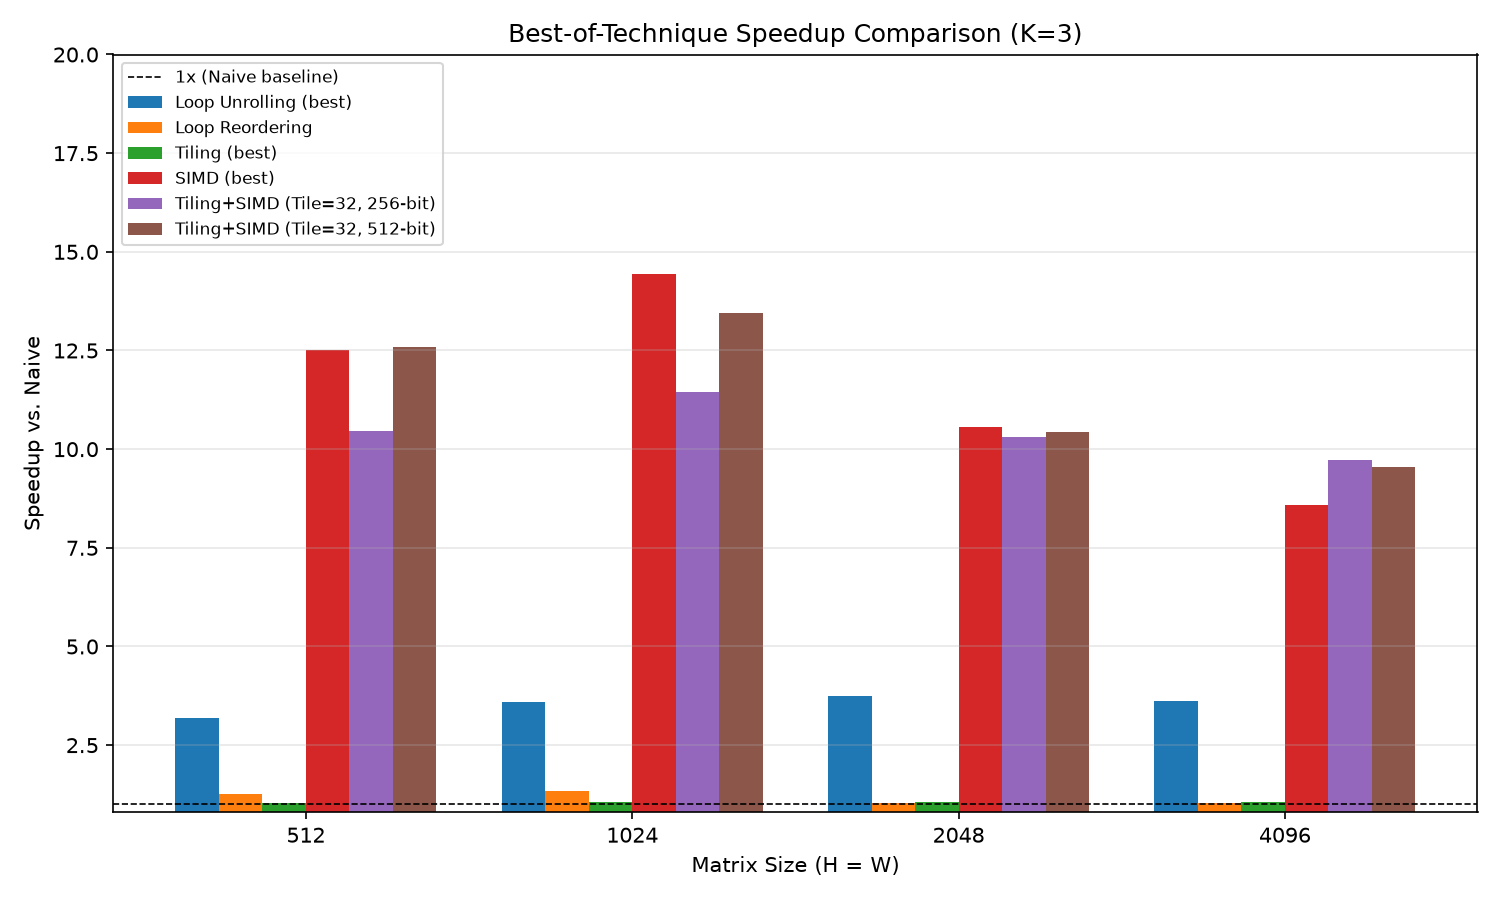
\includegraphics[width=0.9\textwidth]{figures/final_comparison_K3.png}
  \caption{Best-of-technique speedup comparison vs.\ matrix size ($K=3$).}
  \label{fig:final-comparison}
\end{figure}
\begin{figure}[H]
  \centering
  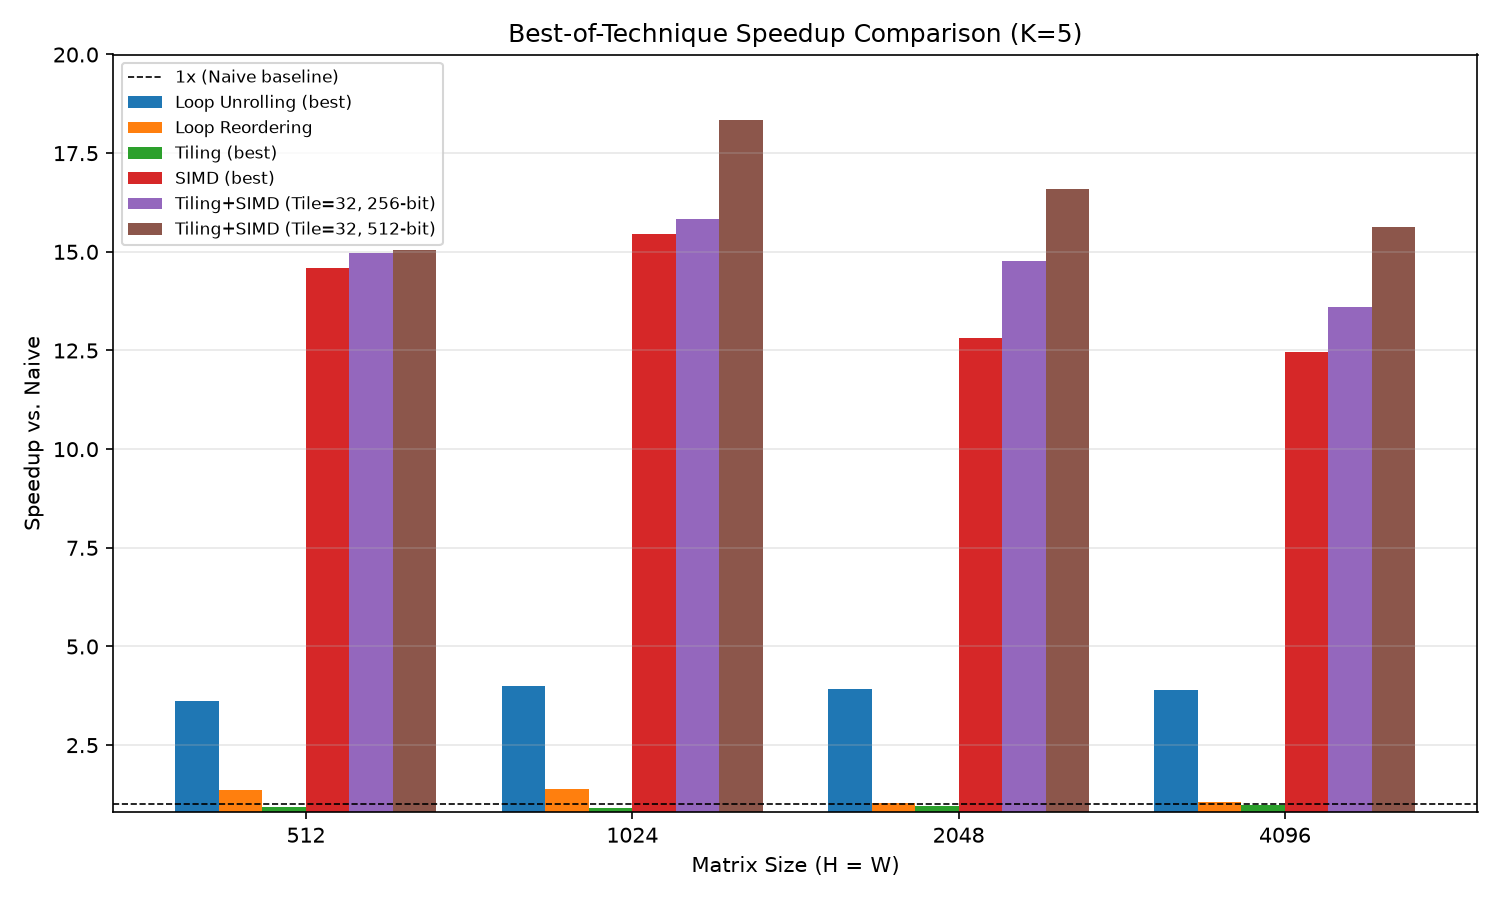
\includegraphics[width=0.9\textwidth]{figures/final_comparison_K5.png}
  \caption{Best-of-technique speedup comparison vs.\ matrix size ($K=5$).}
  \label{fig:final-comparison-k5}
\end{figure}

\end{document}